\documentclass[11pt,a4paper]{article}
\usepackage{od}
\usepackage[utf8]{inputenc}
\usepackage[main=english,russian]{babel}

\title{Inventive problem solving using the\\ OTSM-TRIZ “TONGS” model}

\author{Nikolai Khomenko, John Cooke}
\date{2007 (?)}

\begin{document}
\maketitle
\begin{quote}
  Source: \url{https://otsm-triz.org/sites/default/files/ready/tongs_en.pdf}
\end{quote}

\begin{abstract}
One of the simplest tools in OTSM-TRIZ is the “TONGS” model. Despite being
simple, the “TONGS” model provides a versatile way to frame and study an
inventive technological problem.  For TRIZ novices, the “TONGS” model can be
trained and applied very rapidly.  For more advanced TRIZ users, the “TONGS”
model can set discrete TRIZ tools in context or can direct each process step
in ARIZ (Algorithm for Inventive Problem Solving) and PFN (OTSM based Problem
Flow Networks approach). In this paper we describe the “TONGS” model and apply
it to an inventive problem situation, highlighting the benefits of this
model. Finally, we describe some key applications for the “TONGS” model in
education, problem solving and in the development of new OTSM-TRIZ tools.

\emph{Keywords:} OTSM-TRIZ, TONGS model, Problem Solving
\end{abstract}

\section{Introduction and short history of the\\ TONGS problem solving model:}  

The “TONGS” model is the simplest and most accessible model from Classical
TRIZ and it has the advantage that it can be learned quickly and used by
people who are entirely new to TRIZ, without any deep learning of the theory
and its tools.  At the same time this model was historically the first one
that appeared in the course of Classical TRIZ evolution, starting from the
very simple methodology that was used in the 1940-50s. We believe it can be
useful to introduce this old model to students with modern remarks and
comments and that is why we mention in the paper some of the theoretical
background and tools of Classical TRIZ and OTSM, linking this oldest model
with Classical TRIZ and OTSM and the more recent problem solving process
models and tools based on TRIZ and OTSM. What is surprising is that this model
appears perfectly ready for practical applications of all three postulates of
Classical TRIZ that were formulated later to provide a part of the theoretical
background of Classical TRIZ.

The name of the model first appeared in the course of OTSM evolution; this was
done for educational purposes to help our students communicate efficiently
about the various problem solving process models which are used in Classical
TRIZ and OTSM.

After the “TONGS“ problem solving process model first appeared in TRIZ in the
1940-s [1, 2], it evolved through the introduction of additional rules and
procedures but was not fundamentally changed until after the mid 1970s when
new problem solving process model was implemented for the first time in ARIZ
77. We named it the “HILL” model [3]. This model has a very different
structure from the “TONGS” model but included it as a component. The next
problem solving process model appeared in the middle of 1980-s. We named it
“Problem Flow Model”. It was implemented in ARIZ-85C.  Both previous models
became components of the new model.  In the course of the transition from
Classical TRIZ to OTSM, it appeared that the “PROBLEM FLOW” model included the
three previous models as components.  Finally the “PROBLEM FLOW” model
appeared as a component of the more advanced and universal OTSM Fractal Model
of a problem solving process [4, 5].  This new model is now being used to
create the third generation of the OTSM toolbox, including all previous models
as components. We should mention here just one more model that we call the
“FUNNEL” model.  This problem solving process model of Classical TRIZ is used
for integration of all others into a unified system.  It illustrates the
process of narrowing the area of research we should conduct in order to
develop a satisfactory solution.

We have provided this short history of the evolution of the TRIZ and OTSM
problem solving process models to show why we propose to start the TRIZ
educational process with the “TONGS” model. First of all it is still an active
tool that is a component of the more powerful models and tools. It is simple
to learn and can be developed further to prepare students for deep learning of
Altshuller’s ARIZ.  Step by step the students can learn all of the TRIZ and
OTSM models and how to implement them in particular situations. The “TONGS”
model is also helpful in developing the many skills that they are necessary to
have in order to understand and learn the modern tools of Classical TRIZ and
OTSM.  The “TONGS” model can be viewed also as a “frame” for learning every
single tool, its components and steps more deeply.  This model is not only a
problem solving tool in itself but also a tool for learning many other problem
solving concepts starting right away from the deeply philosophical but still
practical background of classical TRIZ.

\section{How to apply the TONGS model}

According the OTSM Axiom of a root of problems fundamentally, any problem
situation can be described as a conflict between human desire and objective
factors or natural laws. The TONGS model can be used to spell out the
conflicting elements of any problem situation, drill down into the objective
factors preventing us from solving the problem and steer us towards a strong
solution.  Although the TONGS model is simple to apply and use, there are some
key steps which should be followed to get most advantage from the approach.
The sequence of application is not critical but it is important to be
consistent and logical when using the model and to work systematically towards
uncovering the core of the problem.  One last point about the TONGS model is
that it is intended to support an iterative process, where we use partial
solutions to help us to explore the barriers which prevent us from completing
our problem solving journey from our “departure point” to our “final
destination”.  The more competence users have in Classical TRIZ, OTSM and
their related problem solving toolboxes, the less iteration they will need.

\begin{center}
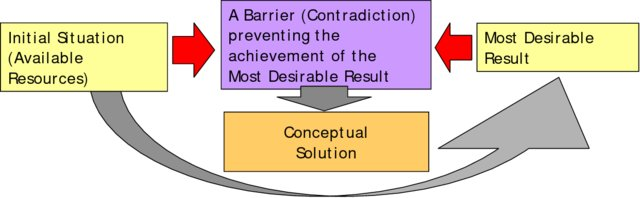
\includegraphics[width=.95\textwidth]{./1.jpg}\\
\textbf{Figure 1:} General schema of The Tongs model of a problem solving
    process.
\end{center}

The key steps in the TONGS model are:

\textbf{2.1 State the Initial Situation (IS):}

This should be a description in simple language (i.e. without professional
jargon and terminology) of the initial problem situation.  The statement
should highlight the main Negative Effect of the problem situation -- in other
words it should describe what it is that seems at the beginning the most
unsatisfactory aspect of the current situation.  As a trivial example, we
could consider the subject of cleaning dishes after a meal, in which case the
main Negative Effect we might state is “it takes a lot of time to clean the
dishesafter a family meal”.

\textbf{2.2 State the Most Desirable Result (MDR):}

This should be a description of the best outcome to the problem situation or
an ideal solution.  The stronger and more provocative we can make the MDR
statement, the more useful it will be in guiding the subsequent problem
solving stages.  To generate a really stretching statement of the Most
Desirable Result, we can imagine that we have in our hand a magic wand which
can be waved over the problem situation to achieve a result that would usually
seem totally impossible to achieve.  Another way to think of the MDR is to
state the positive result that is needed which also eliminates the negative
effect.  To steer the analysis away from more complex solutions, it also helps
to write the MDR statement in such a way that the system with the problem
stays the same (or possibly becomes simpler) while the problem is solved
completely.  It is a good idea to use here the rules of DTC operator to
exaggerate the situation. Do not forget – we have a magic wand!  Everything is
possible on this stage of a problem analysis (according to the OTSM Axiom of
Impossibility)! For the example of cleaning dishes, after exaggeration a bold
statement of the MDR might be “the dishes clean themselves” (or “the dirt
disappears by itself” -- OTSM-TRIZ has rules to make a choice among set of
alternative MDRs. Those rules can be learned later or right away, depending on
the duration of the course).

\textbf{2.3 a) State the Barrier:}

During this stage, we describe what seems most impossible about our statement
of the MDR within the context of the Initial Situation. The purpose of stating
the Barrier in this way is to expose what it is that is stopping us from
achieving the MDR.  At this stage it can be useful to think about the OTSM
axiom of impossibility or in other words, if something “impossible” happens,
how might it practically happen? If the duration of the training course
allows, to answer the question, we can teach students how they can use the
“Gold Fish” method proposed by G. Altshuller or Sword Fish method (to assume
something that that cannot be assumed) developed by V. Gerasimov [6].

In the example of cleaning dishes, we might say that the main Barrier is that
we have no means to make the dishes clean themselves.  One question we can now
start to ask is if we did have self cleaning dishes, how might they clean
themselves?

\textbf{b) Reframe the Barrier as a contradiction:}

Now we drill down into the problem to discover the objective (natural) factor
which is behind the problem we stated in the Initial Situation. This also
helps us to re-state the problem as a new Initial Situation with a new
Negative Effect. To do this we can ask ourselves the question “what is the new
Negative Effect we now have or the new Initial Situation we have to improve?”
In the case of the example of cleaning dishes, the objective factor we need to
address is that without any cleaning action, the food residue will stay stuck
on the dishes. In other words, the Negative Effect we now need to deal with is
the food residue sticking to the dish surface.

\textbf{2.4 a) Identify “Common Sense” Solutions:}

Confronted with the new Negative Effect, we now need to ask ourselves “what
common sense or professional solutions might solve or partially solve this
re-stated problem”. At this stage we don’t need to identify a complete
solution, we simply want to attempt to move closer to the MDR.  In the case of
preventing food residue from sticking to the dish surface, we might suggest a
low-friction coating on the surface of the dish.  This new “common sense”
solution may well have further drawbacks, when tested against the MDR, which
can be used as the basis for a new Initial Situation description which allows
us to iterate through another cycle of the TONGS model.

\textbf{b) Identify OTSM-TRIZ based solutions} using OTSM-TRIZ principles of
contradiction resolution or Classical TRIZ system of Standard Inventive
Solution or any other OTSM-TRIZ based method that the user might know:

If we have more knowledge of TRIZ, we can apply a number of TRIZ tools at this
stage, for example we can answer the following questions:

“What principles of technical contradiction resolution could be useful to
resolve the technical contradictionin this problem?”

“What principles of OTSM-TRIZ could be used to satisfy both opposite demands
for the same parameter?”

“What is the Substance-Field model for this problem situation and which of the
76 Standard Inventive solutions can be used?”

Once again we can test solutions generated during this step against the MDR
and if necessary, use the most appropriate solution for a further cycle
through the TONGS model.

\section{An example of the TONGS model applied to a real problem:}

The problem being solved appeared as a Request for Proposal (RFP) document on
the Nine Sigma website (\url{http://www.ninesigma.com}) in July 2008.

\subsection*{The problem}

Against the background of a need for more fuel efficient vehicles, auto
manufacturers are urgently looking for ways to reduce vehicle weight.  One
area which is under active investigation is the use of aluminium body panels
to replace steel.  Indeed, some car manufacturers such as Audi and Jaguar are
already using the technique on their more expensive models.  In order to form
a body panel, flat sheets of metal are fed from a stack of sheets into a press
(figure~2).\vskip1em

\begin{minipage}{.45\textwidth}\centering
  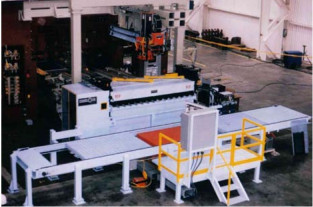
\includegraphics[width=.8\textwidth]{./2.jpg}\\[1em]
  \textbf{Fig. 2:} De-stack sheet feeder system.
\end{minipage}\hfill
\begin{minipage}{.45\textwidth}\centering
  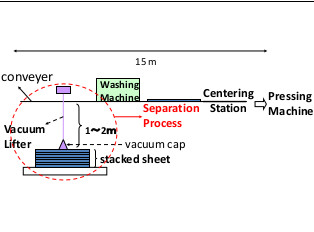
\includegraphics[width=.8\textwidth]{./3.jpg}\\
  \textbf{Fig. 3:} Aluminium sheet feeder layout.
\end{minipage}\vskip1em

Steel sheets can be fed very quickly by this method – as fast as one every two
seconds, but aluminium sheets can only be fed at a rate of 8 per minute. There
are tried and tested methods to separate steel sheets using magnets but these
don’t work for aluminium because it is non-magnetic.  Also, the aluminium
sheets are coated with a sticky oil film, which is needed for a previous
process step and cannot be easily removed.  The Nine Sigma RFP requested
solutions which would allow a doubling of the feed rate for aluminium sheets.
Figure 3 shows the arrangement of the aluminium sheet feeding system.

Application of the TONGS model to this problem:

\textbf{3.1  State the Initial Situation (IS-0):}

In this problem, the Initial Situation is one where the main Negative Effect
is “\emph{if the sheets are fed too quickly, the second sheet sticks to the
  first sheet and stops the press feeder}”.

\textbf{3.2 State the Most Desirable Result (MDR-0): }

For the sheet feeding problem, an MDR we might wish for is that “\emph{as the
  vacuum suckers arrive above the top sheet, the top sheet immediately
  separates itself from the second sheet and moves towards the suckers}”.

\textbf{3.3 a) State the Barrier:}

In this problem, the key barrier seems to be that “\emph{the sheets can’t
  separate themselves because air doesn’t have enough time to get between the
  top sheet and second sheet and atmospheric pressure is holding the two
  sheets together}”.

\textbf{b) Reframe the Barrier} as a contradiction between Human desire and
Natural Laws or other objective factor (OTSM axiom of a root of problems):

In this problem, the objective factor which is at the root of the problem is
that “\emph{it takes a certain amount of time for the air to pass between the
  two sheets but we need this to happen faster}”.

\textbf{3.4 a) Identify “Common Sense” Solutions:}

What common sense or professional solutions might solve or partially solve
this re-stated problem?

A possible partial solution to get air to move more quickly between the two
top sheets is to set up a pressurised air feed to blow air into the gap
between the two sheets.

If we benchmark this solution against the MDR, we can see that while it does
provide a more positive separation of the two top sheets, it also complicates
the system.  To continue the analysis, we will now iterate through the TONGS
model using this partial solution.

\textbf{\emph{Iteration 1:}}

\textbf{3.5 State the Initial Situation (IS-1):}

In this problem, the Initial Situation is one where the main Negative Effect
is “\emph{the air blast system complicates the sheet feeder}”.

\textbf{3.6  State the Most Desirable Result (MDR-1):}

For the sheet feeding problem, an MDR we might wish for is that “\emph{as the
  vacuum suckers arrive above the top sheet, the top sheet immediately
  separates itself from the second sheet and moves towards the suckers
  \underline{without} complicating the system}”.

\textbf{3.7 a) State the Barrier:}

In this problem, the key barrier seems to be that “\emph{I need something to
  force air past the oil and between the two top sheets}”.

\textbf{b) Reframe the Barrier as a contradiction:}

What is the objective (natural) factor which is behind the problem we stated
in the Initial Situation?  Re-state the problem as a new Initial Situation
with a new Negative Effect.

In this problem, the objective factor which is at the root of the problem is
that “\emph{the oil is stopping the air from moving between the two top
  sheets}”.

\textbf{3.8 a) Identify “Common Sense” Solutions:}

A possible partial solution to prevent the oil stopping the air is to get rid
of the oil completely.

If we benchmark this solution against the MDR, we now have a much simpler
solution but we have lost an important function, that is, to protect the
aluminium sheets.  We will now iterate another time through the TONGS model
using this new partial solution.

\textbf{\emph{Iteration 2:}}

\textbf{3.9 State the Initial Situation (IS-2):}

In this problem, the Initial Situation is one where the main \textbf{Negative
  Effect} is “\emph{without an oil coating, the aluminium sheets are not
  properly protected}”.

\textbf{3.10 State the Most Desirable Result (MDR-2 ):}

For the sheet feeding problem, an \textbf{MDR} we might wish for is that
“\emph{as the vacuum suckers arrive above the top sheet, the top sheet
  immediately separates itself from the second sheet and moves towards the
  suckers \underline{without} complicating the system and the aluminium sheets
  are fully protected}”.

As we can see each of the iterations gives us new knowledge on the context of
the particular situation.  So the Tongs model appears to be a tool to apply
the Third postulate of classical TRIZ concerning the context of a specific
situation [4, 7, 8].

\textbf{3.11 a) State the Barrier:}

In this problem, the key barrier seems to be that “\emph{I need something to
  protect the aluminium sheets but I can’t use oil}”.

\textbf{b) Reframe the Barrier as a contradiction:}

In this problem, the objective factor which is at the root of the problem is
that “\emph{the oil should stop the air to protect the sheet surface but
  shouldn’t stop the air from moving between the two top sheets}”.

\textbf{3.12 a) Identify “Common Sense” Solutions:}

A solution direction suggested here is that something needs to happen to the
oil but what could it be?

We will now move onto stage 4 b) to complete the analysis:

\textbf{b) Identify OTSM-TRIZ solutions} using OTSM-TRIZ principles of
technical or physical contradiction resolution or Classical TRIZ system of
Standard Inventive Solution:

“What principles of technical contradiction resolution could be useful to
resolve the technical contradiction in this problem?”

Possible conflicts we have are between \emph{Speed} and \emph{Loss of
  Substance}, \emph{Speed} and \emph{Harmful Effects Acting on the System} and
\emph{Productivity} and \emph{Loss of Substance}.  A principle which seems to
recur is number 35, parameter change.

“What principles of OTSM-TRIZ could be used to satisfy both opposite demands
for the same parameter?”

To indentify a physical contradiction for the oil we can state the useful
action as “protects aluminium sheet” and the harmful action as “stops air
moving between first and second sheets”.

In order to maintain the useful action the oil must be able to flow $\to$
liquid.

In order to prevent the harmful action, to oil must be not able to flow $\to$
solid.

We can separate in time and use “low melting point oil” which can flow over
the sheets to protect them and then solidify before the sheets are put into a
stack so that air can move freely between the sheets. In other words, the
sheets should be coated in wax.

If we benchmark this solution against the MDR, we now have a relatively simple
solution and we can still fully protect the aluminium sheets. For the purpose
of this example, we can now decide to stop the analysis.

\section{Some other applications of the TONGS problem solving process model}

\subsection{Applications for OTSM-TRIZ Education}

There are at least two key points to mention about theapplication of the
“TONGS” model for the OTSM-TRIZ educational process.

First of all, as we discussed at the beginning of the paper, the “TONGS” model
is one of the main sub-component of the other problem solving process models
which were developed in the course of Classical TRIZ and OTSM evolution. This
means that learning the “TONGS” model can be a key first step towards
developing a deep understanding of many other notions, theory and practical
tools which should be known by TRIZ and OTSM practitioners, professionals and
developers.  The model helps us to understand how the theoretical background
can work for practice; how TRIZ based tools can reduce the amount of trial and
error without losing out on quality of the solution for non typical
problematic situation.  The “TONGS” model also serves to help us better
understandhow Altshuller’s three postulates work as practical tools, helping
us to narrow our research to discover the deep root of a problematic situation
and develop an image of a satisfactory solution.  Each iteration of the
“tongs” model adds at least one more detail to the image of Most Desirable
Result as well as understanding and clarification the Initial Situation.

The more students learn about practical application of the three postulates,
the better they can apply many other tools of Classical TRIZ and OTSM.
Depending of the aim of students and teachers we can provide a deep
understanding on how Classical TRIZ works as a theory for creating new tools
for solving various kinds of non typical problems.

The second point is about the structure of the model. Understanding of the
“TONGS” model structure can be used later to study any other OTSM-TRIZ based
tools as well as many other methods.  For example, each tool or method has an
Initial Situation to which it must be applied. Also every single step of ARIZ
or other similar methodshould start with an Initial Situation. Similarly, the
MDR is a statement of the best possible output that should be delivered from
that step or method. Finally, the core of the step is the mechanism to
overcome the barrier that prevents us from obtaining result of the step or
method from our Initial Situation.  This allowed student to understand better
what kind of difficulties (barriers) they face and how they can overcame those
barriers as soon as they try to apply particular step of ARIZ or any other
methodology.

In other words: The “TONGS” model can be viewed not only as a problem solving
tool but as a tool for education and self education.

\subsection{Applications for OTSM-TRIZ Users}

The more deeply the users study how to apply the different TRIZ and OTSM
techniques and methods for effective application of the “Tongs” model, the
better they can use it for many other OTSM-TRIZ based tools.

For instance: the first part of Altshuller’s ARIZ (ARIZ-85C) is based on the
“HILL” model and the third part is based on the “PROBLEM FLOW" model; steps
1.1 and 1.6 is a direct application of the “TONGS“ model; steps 1.2 – 1.5
dedicated to improve and verify the “TONGS“ model that was created on the step
1.1.  When students clearly understand the meaning and practical application
of the “TONGS“ model for study various tools they can better understand
various applications of those tools and how the tools are integrated into
while system. As a result, they can develop their own combination of the tools
for certain particular needs.  In turn this lead to more flexible use of
various tools (not only OTSM and TRIZ based tools) to operate them for complex
interdisciplinary problematic situations according to the OTSM “FRACTAL MODEL“
of a problem solving process.  For instance “TONGS“ model was used for
developing an OTSM interpretation of Altshuller's Law of Completeness of a
Technical System.  In turn this interpretation was used to create OTSM
Negative system technique, OTSM express analysis of an initial situation, OTSM
Network of Problems/Solutions etc.

As we saw in the earlier example, the “TONGS” model can be used to clarify
both the deep root of an Initial Situation and the more detailed image of a
satisfactory solution as close to MDR as possible.  One of the most important
applications of the ”TONGS model is the description of a sub problems that can
be used for creating an OTSM Network of Problems that can then be used to
discover the bottleneck of a problematic situation and for the evaluation of
obtained solutions [9,10].

The “TONGS” model is also important as a tool to split initial problems into
several subproblems to be solved to obtain an appropriate satisfactory
solution [11].  In this application the “TONGS” model can be used for
clarification of the OTSM network of Problems and Solutions as well as an
independent tool to clarify an initial situation during problem solving
process.

\subsection{Applications for OTSM-TRIZ developers and new tools creating.}

When TRIZ and OTSM professionals start using TRIZ and OTSM as a theoretical
basis on which to create new problem solving tools they can apply the ”TONGS”
model to identify barriers that the particular new tools should be able to
overcome in the course of a problem solving process in general.  Then we can
set out to answer the problem by creating new problem solving tools, methods
or techniques or just by clarifying a particular step of an existing method
and tool.

\section{Conclusions}

More than 60 years of using the “TONGS” model in practice for TRIZ based
problem solving makes this model very useful for study by beginners,
professionals and developers of tools for problem solving.  It is a versatile,
domain-free tool that can be used right away for many areas of human activity.

In turn this gives much more freedom to beginners than the study of other
simple empiric tools of classical TRIZ like the matrix and 40 principles that
appeared before TRIZ was formed as a mature theory. With the “TONGS” model,
many simplified tools can be used more effectively because it helps us to pose
the problem correctly before starting to solve it right away. As we know most
beginners try to solve problems right away as soon as they hear the initial
problem description. With the “TONGS” model they learn the importance of the
MDR as a guide to a satisfactory solution which helps decrease the amount of
useless trials and errors. Each iteration with the “TONGS” model leads to a
better description of the MDR and we can pose the problem correctly and apply
appropriate tools. Looked at it in this way, it is difficult to overestimate
the value of the “TONGS” model for the TRIZ and OTSM educational process.

Understanding the “TONGS” model allows professionals to use existing tools
more effectively and to be more fluent in the application of various tools
from the OTSM-TRIZ toolboxes.

For developers of new problems solving tools, the “TONGS” model provides a
framework for specifying requirements for new tools, methods or new steps in
existing tools.  In turn this allows us to pose the problem about the
importance of a new tool and/or process step in a clear form.  When we obtain
a proposal to improve existing tools or create new ones we can use this form
for preliminary evaluation of the proposals we have developed. Of course the
“TONGS” model cannot replace real life evaluation but preliminary evaluation
of the tools can bring some more improvement before testing it to solve real
problems.  Preliminary evaluation is also helpful in developing several
options of the tool with final selection of the best one through practical
application.

Last but not least, we should stress that the “TONGS” model is a powerful
domain-free educational tool for OTSM-TRIZ teachers that allows them to reduce
the overall time needed to educate students to a good professional level.  The
“TONGS” model builds the ability of students to solve problems based on
Classical TRIZ ideology from the very first steps of their education.
Continued use of the model provides a framework for students to learn about
more advanced models and tools for problem solving in terms of both the
problem context and evaluation of very strong solutions.

\section{Summary}

This paper describes the “TONGS” model, one of the very first TRIZ tools, and
discussed how the tool is still very relevant today, being useful for both
TRIZ novices and established TRIZ users. The “TONGS” model provides an
important “frame” for the problem solving process, or sub-steps within a more
complex process, and gives a simple objective means to determine if the
problem solving process is progressing in the right direction.

\section*{References}

\begin{itemize}
\item[{[1]}] Altshuller G.S., Shapiro R.B.  (1956).  Psychology of inventive
  creativity.  Voprosi Psihologii, 6, 37–49.
\item[{[2]}] Altshuller G.S.  (1986).  The history of ARIZ evolution.
  Simferopol. Manuscript (In Russian).
\item[{[3]}] Altshuller G.S. (1975). The Inventive Problem Solving Process:
  fundamental steps and mechanisms.  Manuscript.  (In Russian).
  [\foreignlanguage{russian}{Г.С.  Альтшуллер. Процесс решения изобретательской
      задачи: основные этапы и механизмы. Рукопись. Баку 1975}]
\item[{[4]}] Khomenko N.  (1999). Education Materials for OTSM Development:
  State of Art 1980–1997, LG-Electronics Learning Center, Piangteck, South
  Korea (in English).
\item[{[5]}] Khomenko N.  (2004).  Materials for OTSM modules of the course
  master in innovation design. Strasbourg: INSA.
\item[{[6]}] Gerasimov V.  To assume something that that cannot be assumed.\\ 
  \url{http://www.trizminsk.org/e/212004.htm}. 
\item[{[7]}] Khomenko N., Ashtiany M. (2007).  Classical TRIZ and OTSM as a
  scientific theoretical background for non-typical problem solving
  instruments.  Proceedings of TRIZ-Future 2007, Frankfurt, Germany.
\item[{[8]}] Altshuller G.S.  (1979). The equations of thinking.  (In
  Russian).  [\foreignlanguage{russian}{Г.С.  Альтшуллер.  Формулы
      талантливого мышления. Журнал «Техника и Наука», 1979 No. 3, с. 29-30}.]
\item[{[9]}] Khomenko N., Kaikov I., Shenk, E. (2006).  OTSM-TRIZ Problem
  network technique: application to the history of German high-speed trains.
  Proceedings of the TRIZ-Future 2006, Kortrjik, Belgium.
\item[{[10]}] Khomenko N., De Guio R., Lelait L., Kaikov I. (2007).  A
  Framework for OTSM-TRIZ Based Computer Support to be used in Complex Problem
  Management.  International Journal of Computer Application in Technology
  (IJCAT).  Volume 30 issue 1/2, 2007.
\item[{[11]}] Khomenko N., Kucheriavy D. (2002).  OTSM-TRIZ problem solving
  process: solutions and their classification.  Proceedings of the TRIZ-Future
  2002, Strasbourg, France.
\end{itemize}
\end{document}
